% ==============================================================================
\section{Statistical Inference}%
\label{sec:statistical_inference}
% ==============================================================================

The following introduces the statistical inference techniques used for the
interpretation of results of searches and measurements at the ATLAS experiment.
Among these are methods for parameter estimation and hypothesis testing. They
are used for fitting statistical models to observed data (or pseudodata) and to
make frequentist statements about the presence or absence of a signal.


\subsection{The \textsc{HistFactory} Model}%
\label{sec:histfactory}

The use of binned data
% , usually in the form of histograms,
is widespread for data visualisation and statistical modelling in HEP. Analyses
of collider data typically consider multiple mutually disjoint regions, also
referred to as \emph{channels}, defined by event selections. Each region
consists of a histogram of a discriminating variable with one or more
bins. Events from different signal and background processes, hereafter referred
to as \emph{physics processes}, contribute to these regions. In this context,
\textsc{HistFactory}~\cite{cranmer2012} is the tool used in this thesis for
constructing statistical models for likelihood-based inference. The
\textsc{HistFactory} model is introduced in the following, adopting the notation
of Ref.~\cite{cranmer2012} with few modifications.

Let $\mathcal{C}$ denote the set of channels and $\mathcal{B}_{c}$ the set of
bins of the histogram in channel~$c$. The probability of observing $n_{cb}$
events in bin~$b$ of channel~$c$ is modelled by a Poisson distribution with
probability mass function $\pois(n_{cb}; \nu_{cb})$, where $\nu_{cb}$ denotes
the expected number of events in a given bin. The expectation~$\nu_{cb}$, which
has to be inferred from the observed data, is parameterised
as~\cite{cranmer2012}
\begin{align*}
  \nu_{cb}(\myvec{\alpha}, \myvec{\phi}, \myvec{\gamma}) =
  \sum_{s \in \mathcal{S}_{c}} \, \gamma_{csb} \, \Phi_{cs}(\myvec{\phi}) \, \eta_{cs}(\myvec{\alpha}) \, \sigma_{csb}(\myvec{\alpha}) \,\text{,}
\end{align*}
where $\mathcal{S}_{c}$ is the set of physics processes contributing to
channel~$c$ and the parameters of the model are denoted by
${\myvec{\alpha} = (\alpha_1, \dots, \alpha_n)}$,
${\myvec{\phi} = (\phi_1, \dots, \phi_m)}$, and $\myvec{\gamma}$.\footnote{The
  vector $\myvec{\gamma}$ groups the $\gamma_{csb}$ parameters for all bins.}
The parameters $\myvec{\alpha}$ and $\myvec{\gamma}$ are nuisance parameters
(NPs) with external constraints, which will be introduced shortly.  The
relevance of the four factors $\gamma_{csb}$, $\Phi_{cs}$, $\eta_{cs}$, and
$\sigma_{csb}$ is described in the following~\cite{cranmer2012}:
\begin{itemize}

\item $\sigma_{csb}(\myvec{\alpha})$ is referred to as the \emph{parameterised
    histogram} of process~$s$ in channel~$c$, the index $b$ denoting the bins of
  the histogram. It estimates the expected number of events from process~$s$ in
  channel~$c$ and is usually derived from simulation or control region data. The
  parameterised histogram has additional degrees of freedom, parameterised by
  $\myvec{\alpha}$, to account for uncertainties on the shape of the
  histogram. These degrees of freedom leave the overall normalisation
  $\sum_{b \in \mathcal{B}_{c}} \sigma_{csb}(\myvec{\alpha})$ for a given
  channel~$c$ and process~$s$ unchanged.

\item $\eta_{cs}(\myvec{\alpha})$ represents a normalisation factor applied
  uniformly to all bins of the parameterised histogram for a given process~$s$
  in channel~$c$. The normalisation factor $\eta_{cs}$ cannot vary freely, since
  it is a function of the constrained parameters $\myvec{\alpha}$. This factor
  is included to account for uncertainties on the normalisation of process~$s$
  in channel~$c$.

\item $\Phi_{cs}(\myvec{\phi})$ also represents a normalisation factor applied
  uniformly to all bins of the parameterised histogram for a given process~$s$
  in channel~$c$. However, $\Phi_{cs}$ is the product of \emph{free}
  (unconstrained) normalisation factors given by
  \begin{align*}
    \Phi_{cs}(\myvec{\phi}) = \prod_{p \in \mathcal{N}_{cs}} \phi_p \,\text{,}
  \end{align*}
  where $\mathcal{N}_{cs}$ defines the normalisation factors that are to be
  applied to a given process~$s$ in channel~$c$.
  % These parameters are optional, i.e.\ they can be fixed to unity for a given
  % process/channel depending on the statistical model one wants to construct.
  % % Normalisation factors that are shared?
  In most cases, at least one normalisation factor is present that is applied to
  the physics process of interest, also referred to as the \emph{signal}. This
  normalisation factor is called the \emph{signal strength}~$\mu$ and is usually
  considered to be the parameter of interest (POI). Normalisation factors are
  considered to be NPs if they are not POIs.

\item $\gamma_{csb}$ are parameters that introduce additional degrees of freedom
  for every bin. They are used for incorporating uncertainties from sources that
  are independent between bins. An example of such an uncertainty is the
  statistical uncertainty arising from the use of finite samples of events to
  estimate $\sigma_{csb}$.

  In this thesis, the method by Barlow and Beeston~\cite{barlow1993} is used to
  account for statistical uncertainties on the estimation of $\sigma_{csb}$. To
  reduce the number of parameters of the statistical model, the method is
  simplified as proposed in Ref.~\cite{conway2011} by only considering the
  statistical uncertainty on $\sum_{s \in \mathcal{S}_{c}} \sigma_{csb}$ for a
  given bin and channel. Consequently, the parameters $\gamma_{csb}$ can be
  replaced by $\gamma_{cb}$, omitting the dependence on the physics process.

\end{itemize}
A description of the exact functional form of $\sigma_{csb}(\myvec{\alpha})$ and
$\eta_{cs}(\myvec{\alpha})$ is omitted here but can be found in
Ref.~\cite{cranmer2012}. The likelihood function of the statistical model is
given by
\begin{align}
  L(\myvec{\alpha}, \myvec{\phi}, \myvec{\gamma}) = \Biggl[\,
  \prod_{c \in \mathcal{C}}
  \prod_{b \in \mathcal{B}_{c}}
  \pois\bigl( n_{cb}; \nu_{cb}(\myvec{\alpha}, \myvec{\phi}, \myvec{\gamma}) \bigr)
  \,\Biggr]
  \times L_{\text{ext}}(\myvec{\alpha}, \myvec{\gamma}) \,\text{,}
  \label{eq:likelihood_histfactory}
\end{align}
where $L_{\text{ext}}(\myvec{\alpha}, \myvec{\gamma})$ is the likelihood
function that defines the external constraints on the NPs~$\myvec{\alpha}$ and
$\myvec{\gamma}$. The likelihood
function~$L_{\text{ext}}(\myvec{\alpha}, \myvec{\gamma})$ reads
\begin{align}
  L_{\text{ext}}(\myvec{\alpha}, \myvec{\gamma}) =
  \Biggl[\, \prod_{p=1}^{n} f(a_p; \alpha_p)     \,\Biggr]
  \Biggl[\, \prod_{c \in \mathcal{C}} \prod_{b \in \mathcal{B}_{c}} \pois(m_{cb}; \gamma_{cb} \tau_{cb}) \,\Biggr] \,\text{,}
  \label{eq:likelihood_histfactory_constraints}
\end{align}
with the terms in brackets being described in the following:
\begin{itemize}

\item The term $f(a_p; \alpha_p)$ can be interpreted as the likelihood function
  of an auxiliary measurement of the parameter~$\alpha_p$ given that $a_p$ is
  observed. Conventionally, $f(a_p; \alpha_p)$ is taken to be the probability
  density of a Normal distribution with unit variance and mean
  $\alpha_p$. Furthermore, it is assumed that the measurement observed $a_p = 0$
  such that, considering only the auxiliary measurement, the maximum likelihood
  estimate (MLE) of $\alpha_p$ is 0 with an uncertainty of
  $\Delta \alpha_p = \pm 1$. This particular choice of constraint term is
  closely connected to the functional form of $\sigma_{csb}(\myvec{\alpha})$ and
  $\eta_{cs}(\myvec{\alpha})$. For example, in a model with one externally
  constrained NP the nominal histogram and normalisation is given by
  $\sigma_{csb}(0)$ and $\eta_{cs}(0)$, while $\sigma_{csb}(\pm 1)$ and
  $\eta_{cs}(\pm 1)$ correspond to $\pm 1 \sigma$ variations of the histogram
  shape and normalisation, respectively.

  % which completely describe the physical effects of the nuisance
  % parameter.\footnote{\cite{cranmer2012}.}

\item The $\pois(m_{cb}; \gamma_{cb} \tau_{cb})$ terms provide constraints for
  the $\gamma_{cb}$ parameters introduced by the simplified Barlow--Beeston
  method. For every bin a constant
  $ \tau_{cb} = ( \sum_i w_i )^2 / \sum_i w_i^2 $ is defined, where the sums go
  over events making up the background prediction in the given bin and $w_i$ are
  the corresponding event weights. The constant~$\tau_{cb}$ can be interpreted
  as an effective number of events, which measures the statistical precision of
  the background estimate in the bin.\footnote{Let $Y = \sum_{i = 1}^{N} W_i$
    and $Y^\prime = \sum_{i = 1}^{N^\prime} c$, where $N$ and $N^\prime$ are
    independent Poisson random variables, $W_i$ are i.i.d.\ weights that are
    independent of $N$ and $N^\prime$, and $c$ is a constant. The effective
    number of events refers to the value of $\expect(N^\prime)$ such that
    $\expect(Y) = \expect(Y^\prime)$ and $\var(Y) = \var(Y^\prime)$. This
    condition yields
    $\expect(N^\prime) = \expect(N) \expect(W)^2 / \expect(W^2)$, and after
    approximating expected values with sample averages
    $\expect(N^\prime) \approx ( \sum_i w_i )^2 / \sum_i w_i^2$.} The model
  incorporates the statistical uncertainty by setting up auxiliary measurements
  of the effective number of events, $\gamma_{cb}\tau_{cb}$, for every
  bin. These measurements observe $m_{cb} = \tau_{cb}$, and therefore the
  nominal value of the $\gamma_{cb}$ parameters is 1. Supplementary information
  on the Barlow--Beeston method is given in \Cref{app:barlow_beeston}.

\end{itemize}

Given observed data, the parameters of the model can be estimated using maximum
likelihood estimation. Hereafter, it is assumed that the model has one POI,
namely, the signal strength~$\mu$. All other parameters of the model are
collectively referred to as $\myvec{\theta}$. Let $\Omega$ be the parameter
space of the model with elements~$(\mu, \myvec{\theta})$. The MLE of the
parameters is determined by the \emph{unconditional fit}
\begin{align}
  (\muhat, \hat{\myvec{\theta}}) = \argmax_{(\mu, \myvec{\theta}) \in \Omega} L(\mu, \myvec{\theta}) \,\text{.}
  \label{eq:unconditional_fit}
\end{align}
Often, a restricted model is constructed by fixing the POI to an arbitrary value
$\mu^*$. In this case, the MLE of the model parameters is given by the
\emph{conditional fit for $\mu = \mu^*$}
\begin{align}
  \hat{\hat{\myvec{\theta}}}(\mu^*) = \argmax_{\myvec{\theta} \in \{ \myvec{\theta}^\prime \mid (\mu^*, \myvec{\theta}^\prime) \in \Omega \} } L(\mu^*, \myvec{\theta}) \,\text{.}
  \label{eq:conditional_fit}
\end{align}
The model with the restriction $\mu = 0$ is called the \emph{background-only
  model}, while the unrestricted model is called the
\emph{signal-plus-background model}.

Lastly, special datasets referred to as \emph{Asimov
  datasets}~\cite{Cowan:2010js} are introduced. For a given set of model
parameters, the Asimov dataset is the dataset in which the observables $n_{cb}$
and the global observables $a_p$ and $m_{cb}$ are equal to their expected
values. Asimov datasets can be used, in place of the observed data, to evaluate
the expected experimental sensitivity of searches and measurements in HEP. Some
uses of Asimov datasets are highlighted in subsequent sections.


\subsection{Hypothesis Testing in Particle Physics}%
\label{sec:hypotesting}

In HEP, one is often concerned with comparing the goodness of fit of competing
statistical models to observed data. These comparisons assist in making
statements about values of the signal strength that are still in agreement with
the observations. The framework of statistical hypothesis testing provides a
principled approach to perform these comparisons.

With the statistical model introduced previously, a null hypothesis, $H_0$, is
defined as
\begin{alignat*}{3}
  &H_0: (\mu, \myvec{\theta}) \in \Omega_0
    \quad &\text{with} \quad &\Omega_0 \subset \Omega \,\text{,} \\
  \intertext{where $\Omega_0$ is the set of model parameters that specify the
  null hypothesis, and an alternative hypothesis, $H_1$, is defined as}
  &H_1: (\mu, \myvec{\theta}) \in \Omega_1
    \quad &\text{with} \quad &\Omega_1 = \Omega \setminus \Omega_0 \,\text{.}
\end{alignat*}
% \begin{align*}
%   H_1: (\mu, \myvec{\theta}) \in \Omega_1
%   \quad \text{with} \quad \Omega_1 = \Omega \setminus \Omega_0 \,\text{.}
    %   \end{align*}
%
% \footnote{Example: Taking the background-only hypothesis as
%   the null hypothesis, then $\Omega_0 = \{ (\mu^\prime, \myvec{\theta}^\prime) \in \Omega \mid \mu^\prime = 0 \}$.}
%
A \emph{likelihood ratio test} (LRT) can be used to compare these
hypotheses. The test statistic of the LRT is given by~\cite{casella2001}
\begin{align*}
  \Lambda = -2 \ln\mathopen{}\left[
  \frac{\sup_{(\mu, \myvec{\theta}) \in \Omega_0} L(\mu, \myvec{\theta})}
  {\sup_{(\mu, \myvec{\theta}) \in \Omega\phantom{_0}} L(\mu, \myvec{\theta})}
  \right]\mathclose{} \,\text{,}
\end{align*}
where the numerator (denominator) of the term in brackets is the supremum of the
likelihood for the restricted (unrestricted) model. A critical value of the test
statistic, $\Lambda_{\text{crit}}$, is chosen and compared to the observed value
of the test statistic. If $\Lambda > \Lambda_{\text{crit}}$ then $H_0$ is
rejected in favour of $H_1$. Otherwise, $H_0$ cannot be rejected. The chosen
value of $\Lambda_{\text{crit}}$ defines the rejection region of the test and
thus its significance level and power.


\subsubsection{Discovery of a Signal}

In the context of statistical hypothesis testing, the discovery of a signal
implies rejecting the background-only hypothesis in favour of the
signal-plus-background hypothesis. Generally, only signals with positive
strength, that is $\mu > 0$, are considered as potential discoveries. The
relevant hypotheses for testing the discovery of a signal are
\begin{align*}
  &H_0: (\mu, \myvec{\theta}) \in \{ (\mu^\prime, \myvec{\theta}^\prime) \in \Omega^+ \mid \mu^\prime = 0 \}
  &&H_1: (\mu, \myvec{\theta}) \in \{ (\mu^\prime, \myvec{\theta}^\prime) \in \Omega^+ \mid \mu^\prime > 0 \} \,\text{,}
\end{align*}
where $\Omega^+$ denotes the parameter space of the model with the restriction
that $\mu \geq 0$. An empirical test statistic based on the LRT is defined
as~\cite{Cowan:2010js}
\begin{align}
  q_0 = \begin{cases}
          -2 \ln\mathopen{}\left[ \frac{ L\bigl(0, \hat{\hat{\myvec{\theta}}}(0) \bigr)}{L\bigl( \muhat, \hat{\myvec{\theta}} \bigr)} \right]\mathclose{}, & \muhat > 0 \\
          0,          & \muhat \leq 0
        \end{cases} \quad\text{,}
  \label{eq:discovery_teststat}
\end{align}
where $\muhat$, $\hat{\myvec{\theta}}$, and $\hat{\hat{\myvec{\theta}}}$ are
defined as in \Cref{eq:unconditional_fit,eq:conditional_fit}.\footnote{The
  unconditional fit is performed without the $\mu \geq 0$ constraint. Instead,
  the constraint is imposed in the definition of the test statistic by setting
  the maximum likelihood of the unrestricted model to
  $L\bigl( 0, \hat{\hat{\myvec{\theta}}}(0) \bigr)$ in the $\muhat < 0$ case.}
This test statistic is referred to as the \emph{discovery test statistic}. The
asymptotic sampling distribution of $q_0$ under $H_0$ is given by the
probability density function~\cite{Cowan:2010js}
\begin{align*}
  f(q_0) = \frac{1}{2} \delta(q_0) + \frac{1}{2} f_{\chi^2}(q_0; 1) \,\text{,}
\end{align*}
which is an equal mixture of a Dirac $\delta$ distribution and a $\chi^2$
distribution with one degree of freedom. The discovery test statistic is often
expressed in terms of an asymptotic $p$-value according to~\cite{Cowan:2010js}
\begin{align*}
  p_0 = \int_{q_{0}}^\infty \mathrm{d}q_0^\prime \, f(q_0^\prime) =
  1 - \Phi\left(\sqrt{q_{0}}\right) \,\text{,}
\end{align*}
where $\Phi$ is the cumulative distribution function of the Standard Normal
distribution. Another way of expressing the test statistic is in terms of the
\emph{discovery significance}~$Z_0$, which is defined as~\cite{Cowan:2010js}
\begin{align*}
  Z_0 = \Phi^{-1}(1 - p_0) = \sqrt{q_{0}} \,\text{.}
\end{align*}
In particle physics, the conventional significance threshold that has to be
exceeded to claim discovery of new physics is $Z_0 = 5$ ($p_0 = \num{2.87e-7}$),
which is also called the ``$5\sigma$ threshold''. Lastly, the \emph{median
  discovery significance} of a signal with an assumed strength of $\mu$ can be
estimated by determining $Z_0$ for an Asimov dataset constructed with the same
signal strength~\cite{Cowan:2010js}. The median discovery significance is also
referred to as the \emph{expected signal significance}.


\subsubsection{Upper Limits on the Signal Strength}

Often, one is interested in determining the largest signal strength that would
still be compatible with the observed data. Formally, this constitutes
estimating a one-sided confidence interval for $\mu$ that is bounded from above,
hence referred to as an upper limit. The upper limit can be obtained by
inverting a test of the hypotheses
\begin{align*}
  &H_0: (\mu, \myvec{\theta}) \in \{ (\mu^\prime, \myvec{\theta}^\prime) \in \Omega^+ \mid \mu^\prime \geq \mu^* \}
  &&H_1: (\mu, \myvec{\theta}) \in \{ (\mu^\prime, \myvec{\theta}^\prime) \in \Omega^+ \mid \mu^\prime < \mu^* \} \,\text{,}
\end{align*}
where $\mu^*$ is used to parameterise the hypotheses. Let $1 - \alpha$ be the
desired confidence level (CL) of the interval to be estimated. Given a test of
$H_0$ and $H_1$ with significance level~$\alpha$, the confidence interval is the
set of values of $\mu^*$ for which $H_0$ cannot be rejected by the test. The
upper bound of this set is
% referred to as
the upper limit on $\mu$ at $1 - \alpha$~CL.

The estimation of upper limits in HEP uses an empirical test statistic derived
from the LRT that reads~\cite{Cowan:2010js}
\begin{align}
  \qmutilde =
  \begin{cases}
    -2\ln\mathopen{}\left[ \frac{ L\bigl( \mu, \hat{\hat{\myvec{\theta}}}(\mu) \bigr)}{L\bigl( 0, \hat{\hat{\myvec{\theta}}}(0) \bigr)} \right]\mathclose{}, & \muhat \in (-\infty, 0] \\[1em]
    -2\ln\mathopen{}\left[ \frac{ L\bigl( \mu, \hat{\hat{\myvec{\theta}}}(\mu) \bigr)}{L\bigl( \muhat, \hat{\myvec{\theta}} \bigr)} \right]\mathclose{}, & \muhat \in (0, \mu] \\[1em]
    0,\phantom{ \biggl[  \biggr]} & \muhat \in (\mu, \infty) \\
  \end{cases} \,\text{,}
  \label{eq:qmutilde}
\end{align}
where for notational simplicity $\mu^*$ is replaced by $\mu$. Moreover, the
unconditional fit determining $\muhat$ and $\hat{\myvec{\theta}}$ in
\Cref{eq:qmutilde} is performed without the positivity constraint on the signal
strength. The asymptotic sampling distribution of \qmutilde was derived in
Ref.~\cite{Cowan:2010js} for any assumed value of the true signal strength.
Let~$f(\qmutilde \mid \mu^\prime)$ be the asymptotic sampling distribution of
\qmutilde under the assumption that the signal strength is
$\mu^\prime$. Following the approach outlined before, an upper limit at
$1 - \alpha$~CL can be determined by finding the largest value of $\mu$ such
that
\begin{align*}
  p_\mu = \int_{\tilde{q}_{\mu, \text{obs}}}^{\infty} \mathrm{d}\qmutilde \, f(\qmutilde \mid \mu) > \alpha \,\text{,}
\end{align*}
where $\tilde{q}_{\mu, \text{obs}}$ denotes the observed value of the test
statistic. Confidence intervals derived using this method have an asymptotic
coverage probability of $1 - \alpha$.

Searches for new physics use the \CLs~technique
~\cite{Junk:1999kv,Read:2000ru,Read:2002hq} to set upper limits on $\mu$
instead. To motivate the use of this technique, a problem with tests based
on~$p_\mu$ is outlined hereafter. A test of $H_0: \mu \geq \mu^*$ and
$H_1: \mu < \mu^*$ with rejection region~$p_{\mu^*} \leq \alpha$ has an
asymptotic significance level of~$\alpha$ by construction.
% Consequently, the probability of falsely rejecting $H_0$ when $\mu = \mu^*$ is $\alpha$.
Since $\alpha$ is fixed a priori, the probability/power of correctly
rejecting~$H_0$ under the background-only hypothesis, denoted by $1 - \beta$, is
solely determined by the experimental sensitivity to a signal with
strength~$\mu^*$. This is illustrated in
\Cref{fig:cls_qmu_highpower,fig:cls_qmu_lowpower} for an experiment with high
and low sensitivity, respectively. A problem arises when considering an
experiment that has little sensitivity in distinguishing between the
$\mu = \mu^*$ and $\mu = 0$ hypotheses. In this case, the power of the
test~($1 - \beta$) approaches $\alpha$, which is illustrated
in~\Cref{fig:cls_qmu_lowpower}. This means that a signal to which the experiment
has no sensitivity will still be excluded with a probability of at
least~$\alpha$ under the background-only hypothesis. In HEP, such \emph{spurious
  exclusions} are not desired, motivating the use of an alternative method for
setting upper limits that takes into account the signal sensitivity of the
experiment.

\begin{figure}[htbp]
  \centering

  \begin{subfigure}{0.46\textwidth}
    % 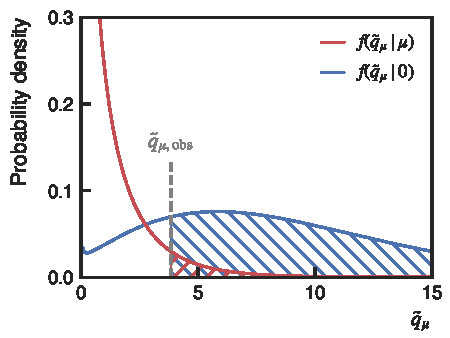
\includegraphics[width=\textwidth]{statistics/cls_high_sensitivity}
    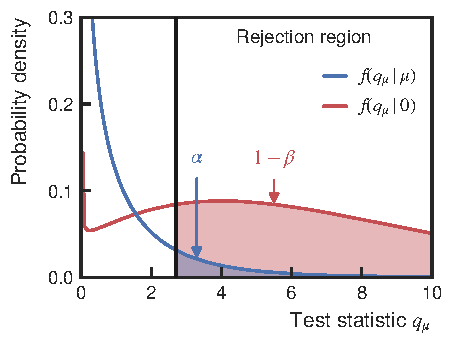
\includegraphics[width=\textwidth]{statistics/high_power}
    \caption{Test with high statistical power ($1 - \beta = 0.8$).}%
    \label{fig:cls_qmu_highpower}
  \end{subfigure}\hfill%
  \begin{subfigure}{0.46\textwidth}
    % 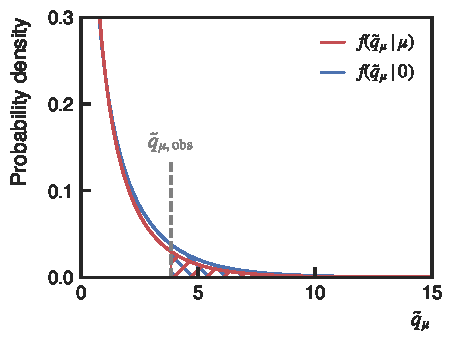
\includegraphics[width=\textwidth]{statistics/cls_low_sensitivity}
    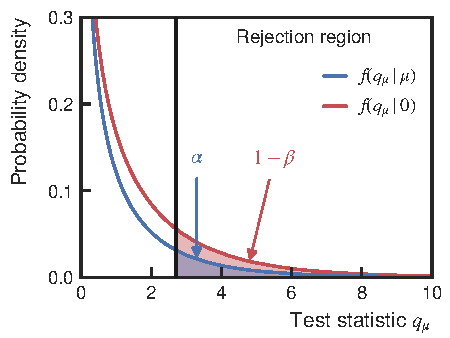
\includegraphics[width=\textwidth]{statistics/low_power}
    \caption{Test with low statistical power ($1 - \beta = 0.1$).}%
    \label{fig:cls_qmu_lowpower}
  \end{subfigure}

  \caption[Sampling distribution of the test statistic for upper limits under
  the signal-plus-background and background-only hypothesis.]{Sampling
    distribution of $q_{\mu}$ under the signal-plus-background (blue) and
    background-only (red) hypothesis. The area shaded in blue corresponds to the
    significance level~$\alpha$ of the test, which is $\alpha = 0.05$ in both
    cases. The area shaded in red corresponds to the statistical
    power~$1 - \beta$ of the test. The test statistic
    $q_{\mu}$~\cite{Cowan:2010js}, which differs from \qmutilde by allowing
    negative values of the signal strength, is chosen for illustration purposes
    only.}%
  \label{fig:cls_qmu}
\end{figure}

The \CLs technique addresses the problem of spurious exclusions by introducing
the test statistic~\cite{Cowan:2010js}
\begin{align*}
  \CLs = \frac
  {\int_{\tilde{q}_{\mu, \text{obs}}}^{\infty} \mathrm{d}\qmutilde \, f(\qmutilde \mid \mu)}
  {\int_{\tilde{q}_{\mu, \text{obs}}}^\infty \mathrm{d}\qmutilde \, f(\qmutilde \mid 0)} \,\text{.}
  % \label{eq:cls}
\end{align*}
This statistic modifies $p_\mu$ (the numerator) by dividing it by the
probability of \qmutilde being larger than the observed value under the
background-only hypothesis. Upper limits on the signal strength are then
estimated by finding the largest value of $\mu$ for which $\CLs > \alpha$. In
the limiting case of an experiment with no signal sensitivity the value of \CLs
approaches unity, thus preventing spurious exclusions. Limits derived using this
approach are also referred to as upper limits at $1 - \alpha$~CL; however, their
coverage probability exceeds $1 - \alpha$ by construction due to $\CLs >
p_\mu$. Therefore, confidence intervals estimated using the \CLs technique are
considered to be conservative. By convention, upper limits on $\mu$ are set at
$\SI{95}{\percent}$~CL ($\alpha = 0.05$) in HEP. Lastly, the \emph{median upper
  limit} on $\mu$ can be derived by performing the procedure using
background-only Asimov data instead of the observed
data~\cite{Cowan:2010js}. The median upper limit is also referred to as the
\emph{expected upper limit}. An example of the limit setting procedure using the
\CLs method is given in \Cref{fig:cls_example}. All upper limits in the
remainder of this thesis are determined using the \CLs~technique.

\begin{figure}[htbp]
  \centering

  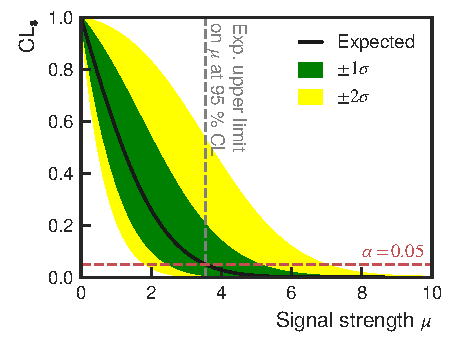
\includegraphics[width=0.46\textwidth]{statistics/cls_limits}

  \caption[The \CLs test statistic as a function of $\mu$ for an event counting
  experiment.]{The \CLs test statistic as a function of~$\mu$ for an event
    counting experiment with an expectation of 5 signal events, 50 background
    events, and a background systematic uncertainty of \SI{10}{\percent}. The
    expected/median \CLs is obtained from the background-only Asimov
    dataset. The \CLs intervals containing approximately
    \SI{68}{\percent}~($\pm 1 \sigma$) and \SI{95}{\percent}~($\pm 2 \sigma$) of
    probability mass are indicated as coloured bands.}%
  \label{fig:cls_example}
\end{figure}

%%% Local Variables:
%%% mode: latex
%%% TeX-master: "../../phd_thesis"
%%% End:
